

The main goal of our fast path  is to forgo the overhead associated with two-phase transaction processing, especially for short transactions.
In particular, the fast path can eliminate the need for remote access in local (single-region) transactions and can reduce the number of 
calls (RPCs) the client performs.
To this end, we introduce in Section~\ref{ssec:fast-api} a streamlined API that jointly executes multiple API calls of the original TPS. 
We refer to transactions that use this API as \emph{fast path (FP) transactions}.
We discuss the semantics of FP transactions relative to regular ones in Section~\ref{ssec:fast-semantics}.

\subsection{API and usage}
\label{ssec:fast-api}

For brevity, we refer to the TPS's API calls  begin, read, write, and commit as \code{b, r, w}, and \code{c} respectively. 
We now combine them to allow fast processing.
The simplest examples of FP transactions are singletons, i.e., transactions that perform a single
read or write. These are supported by the APIs:
\begin{description}
\item[br(key)] -- begins an FP transaction and reads key within it. Recall that read-only transactions need not commit. 
\item[bwc(key,val)] -- begins an FP transaction,  writes val into a new version of key that exceeds all existing ones, and commits.
\end{description}

A more elaborate example is a read-modify-write API: 
\begin{description}
\item[brwc(key,)] -- begins an FP transaction,  reads the latest version of key, applies $f$ to it (on the server side), 
	writes the result into a new version of key that exceeds all existing ones, and commits.
\end{description}

To use the above API, the programmer has to encapsulate the transaction logic in a function for server-side processing. 
Alternatively, we allow FP transactions to unfold dynamically much like regular  transactions do.
A dynamic FP transaction may instead begin with a \code{br} call, perform client-side processing, and then call the following
function to update either the same or a different key: 

\begin{description}
\item[wc(key,val)] -- writes val into a new version of key that exceeds all existing ones, and commits.
\end{description}

Moreover, we do not restrict FP transactions to perform a single read -- any number of \code{r}'s may be called between the \code{br} 
and \code{wc}. The supported types of FP transactions are summarized in Table~\ref{table:fp-types}.
Note, however, that all calls must be directed at the same region, else the transaction is not local.
In case an FP transaction dynamically discovers that it needs to access additional regions, it is aborted and should be restarted as a regular transaction. 

\begin{table}[htb]
%\def\arraystretch{1.5}%  1 is the default, change whatever you need
\centerline{
\begin{tabular}{l  @{\hspace{2em}} l}
Call sequence & Transaction type\\
\hline
\code{br} & single read\\
\code{bwc} & single write\\
\code{br, r*} &  multi-read\\
\code{br, r*, wc} & multi-read, single write\\
\code{brwc} & server-side single-read-write\\
%\hline
\end{tabular}
}
\caption{Supported FP transaction types.}
\label{table:fp-types}
\end{table}

In principle, it would have been possible to also allow \code{w} calls in the span of an FP transaction, 
but in this case, it is not possible to forgo the two-phase execution. 
That is, the \code{w} calls would need to indicate write intents, and  to be atomically committed (or aborted) during the final \code{wc} 
(or \code{c}) call. 
Given the limited benefit and extra compexity of allowing many writes in FP transactions, we do not support this option in our solution.


\subsection{Semantics}
\label{ssec:fast-semantics}

The semantics for ordering FP transactions relative to regular ones are
weaker than SI in that they do not guarantee real-time order over all regular
and FP transactions together. Specifically, a regular transaction overlapping
two FP ones that access different regions may observe an update of
the second and miss an update by the first. For example, assume objects $x$ and $y$
are managed in two different regions, then real-time order can be violated as
illustrated in Figure~\ref{fig:ltx-rt} (ignore the skip operations for now; they will be explained in the next section).

\begin{figure}[h]
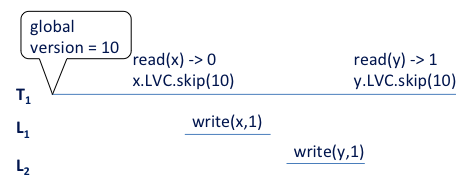
\includegraphics[width=\columnwidth]{LTX-RT}
\caption{Possible violation of real-time order among fast path (FP) transactions in different regions. Global transaction $T_1$
reads $x$ before it is updated by FP transaction $FP_1$ and reads $y$ after it is updated by FP transaction $FP_2$ even 
though $FP_2$ occurs after $FP_1$. $T1$'s global version is $10$, and its skips the local version clocks of the regions holding $x$ and $y$ to $10$ when reading from them.}
\label{fig:ltx-rt}
\end{figure}

The system still enforces a total order ${\cal T}$ on all committed transactions, so that
\begin{enumerate}
    \setlength{\itemsep}{0pt}
    \setlength{\parskip}{0pt}
    \setlength{\parsep}{2pt}  
\item
regular transactions (though not FP ones) are ordered in ${\cal T}$  according to their commit times;
\item
FP transactions within each region are ordered in ${\cal T}$  according to their commit times;
\item
each transaction's read operations see a consistent snapshot of the database reflecting 
a prefix of  ${\cal T}$ that includes all transactions committed prior to
its start time plus any number of concurrent FP transactions; and 
\item
 a transaction commits only if none of the items it updates has been modified since that snapshot.
 \end{enumerate}

Note that since ${\cal T}$  respects commit times in each region, causality is preserved, because 
only transactions that  access disjoint  sets of data objects can be re-ordered.


